% !TeX encoding = UTF-8
% !TeX program  = xelatex

\documentclass[12pt,a4paper,openany]{book} 
\usepackage[typeblock=golden]{stb-titlepage}        

%==== Math setup =====================================================
\usepackage{amsmath}%............................. Advanced math (before fonts)
%\usepackage{amssymb}%............................ AMS Symbol fonts

%==== Font setup =====================================================
\usepackage{iftex}
\ifxetex
    \usepackage[math-style=TeX,
                bold-style=TeX,
               ]{unicode-math}
    \setmainfont{Cambria}%........................ Unicode fonts  (Win)                
    \setsansfont[Scale=MatchLowercase]{Calibri}
    \setmonofont[Scale=MatchLowercase]{Consolas}
    \setmathfont{Cambria Math}
    \defaultfontfeatures{Ligatures=TeX}
    \let\bm\symbfit
\else
    \usepackage[utf8]{inputenc}%.................. Unicode file format
    \usepackage{textcomp}%........................ Additional text symbols
    \usepackage[T1]{fontenc}%..................... Type 1 outline fonts
    \usepackage{bm}%.............................. Bold math fonts
\fi
\normalfont

%==== Units and numbers ==============================================
\usepackage{siunitx}%............................. Unit, number and angle output
    \sisetup{detect-all = true, detect-family = true}
    \sisetup{output-decimal-marker = {.} ,
             group-separator = {\,},
             number-unit-product = {\,},
             inter-unit-product = \mathord{\cdot},
             exponent-product = \mathord{\times},
             separate-uncertainty = true}
         
%==== Ref's, Bib's and Nomencl =======================================
\usepackage{stb-nomencl}%......................... List of symbols 
    \renewcommand*{\UnitLabel}[1]{~[\,\unit{#1}\,]}
\usepackage{stb-bib}%............................. Bibliography (natbib internally)
    \bibliographystyle{stb-bib-eng-a}
    \renewcommand\bibfont{\small}
    \renewcommand\bibsection{\chapter{\bibname}}

%==== Tables + Graphics + Color =====================================
\usepackage{array}%............................... Extended table defs 
    \setlength{\extrarowheight}{2pt}
\usepackage{longtable}%........................... Tables can break over pages
\usepackage{graphicx}%............................ Included graphics
\usepackage[font=small]{caption}%................. Customize captions  
\usepackage[table]{xcolor}%....................... Color setup + colortbl 
\usepackage{float}

%==== Extra defs for template ========================================
\makeatletter
%---- TOC entries and case
    \renewcommand\contentsname{Table of contents}
    \renewcommand\listfigurename{List of figures}
    \renewcommand\listtablename{List of tables}
    \renewcommand\bibname{List of references}
    
    \renewcommand\tableofcontents{\chapter*{\contentsname}\@starttoc{toc}}
    \renewcommand\listoffigures{\chapter{\listfigurename}\@starttoc{lof}}
    \renewcommand\listoftables{\chapter{\listtablename}\@starttoc{lot}}

%---- Plagiarism signatures
    \newcommand\tstrut[1][4ex]{\rule{0pt}{#1}}
    \newcommand\tdots[1][5cm]{\makebox[#1]{\dotfill}}

%---- Summary head line
    \newcommand\sumheading{%
        \rowcolor[gray]{.9}%
        \centering\arraybackslash%
        \bfseries\normalsize}

%==== User Defs ======================================================
%
% Please insert user defined commands here
% and NOT in the document itself!
%
%
\makeatother

%==== Title Page =====================================================
\title{\textbf{Development of a Hydrogel Extruder}\\[2ex]
       \large Mechatronic Project 478\\Final Report\\[2ex]}                   
\author{\Large Author: Simon Craig Daniel\\ 
        \large 25848887 \\[5ex]
        \Large Supervisor: Mr. Wayne Swart}                
\address{Department of Mechanical and Mechatronic Engineering\\
        Stellenbosch University \\
        Private Bag X1, Matieland 7602, South Africa.}
\date{2025/01/05}                             
\Copyright{2025}{Stellenbosch University.\\ All rights reserved.}

%==== Main Document ==================================================
\setcounter{secnumdepth}{3}
\setcounter{tocdepth}{2}
\raggedbottom
\begin{document}   

\frontmatter%---------------------------------------------------------                    
\maketitle 

\chapter*{Plagiarism declaration}

I have read and understand the Stellenbosch University Policy on Plagiarism and the definitions of plagiarism and self-plagiarism contained in the Policy [Plagiarism: The use of the ideas or material of others without acknowledgement, or the re-use of one's own previously evaluated or published material without acknowledgement or indication thereof (self-plagiarism or text-\-re\-cyc\-ling)].

I also understand that direct translations are plagiarism, unless accompanied by an appropriate acknowledgement of the source. I also know that verbatim copy that has not been explicitly indicated as such, is plagiarism.

I know that plagiarism is a punishable offence and may be referred to the University's Central Disciplinary Committee (CDC) who has the authority to expel me for such an offence.

I know that plagiarism is harmful for the academic environment and that it has a negative impact on any profession.

Accordingly all quotations and contributions from any source whatsoever (including the internet) have been cited fully (acknowledged); further, all verbatim copies have been expressly indicated as such (e.g. through quotation marks) and the sources are cited fully.

I declare that, except where a source has been cited, the work contained in this assignment is my own work and that I have not previously (in its entirety or in part) submitted it for grading in this module/assignment or another module/assignment.
I declare that have not allowed, and will not allow, anyone to use my work (in paper, graphics, electronic, verbal or any other format) with the intention of passing it off as his/her own work.

I know that a mark of zero may be awarded to assignments with plagiarism and also that no opportunity be given to submit an improved assignment. 
\vspace{1.5cm}

\noindent
\begin{tabular}{@{}lllll@{}}
\tstrut Signature: &\tdots&	           &            \\
\tstrut Name:      &\tdots& Student no:&\tdots[3cm] \\
\tstrut Date:      &\tdots&            &            \\
\end{tabular}
		

\chapter*{Executive summary}

\chapter*{ECSA self-assessment}


\chapter*{Acknowledgements}




% Use \chapter*{} before TOC
\tableofcontents
% Use \chapter{} after TOC

\listoffigures
\listoftables
\chapter{List of symbols}
% Use stb-nomenclature + siunitx

\begin{Nomencl}[1cm]
\NomGroup{Constants}%-----------------------------------------------
    \item[$L_0 = $] \qty{300}{mm}

\NomGroup{Variables}%-----------------------------------------------
    \item[$\mathit{Re}_\mathrm{\,D}$]
                       \UnitLine{Reynolds number (diameter)}{~}
    \item[$x$]         \UnitLine{Coordinate                }{m}
    \item[$\ddot{x}$]  \UnitLine{Acceleration              }{m/s^2}\\
    
    \item[$\theta$]    \UnitLine{Rotation angle            }{rad}
    \item[$\tau$]      \UnitLine{Moment                    }{N.m}

\NomGroup{Vectors and Tensors}%-------------------------------------
    \item[$\overrightarrow{\bm{v}}$] Physical vector, see equation ...

\NomGroup{Subscripts}%----------------------------------------------
    \item[$\mathrm{a}$] Adiabatic
    \item[$a$]          Coordinate

\end{Nomencl}

\begin{Nomencl}[1cm]
\NomGroup{Abreviations}%-----------------------------------------------
    \item[DEM] Discrete Element Method
    \item[FEA] Finite Element Analysis

\end{Nomencl}


\mainmatter%----------------------------------------------------------
\numberwithin{figure}{chapter}
\numberwithin{table}{chapter}

\chapter{Introduction}

\section{Background}

Starting from the big picture, gradually narrow focus down to this project and where this report fits in.

\section{Objectives}

The objectives of the project (in some cases the objectives of the report). If necessary describe limitations to the scope.

\section{Motivation}

Why this specific project/report is worthwhile.


\chapter{Literature review}

\section{Tissue engineering}
\subsection{Definition and Background of Tissue Engineering}
Tissue engineering can be defined as the “the application of principles and methods of engineering and life sciences toward fundamental understanding of structure–function relationships in normal and pathological mammalian tissues and the development of biological substitutes to restore, maintain, or improve tissue function” \citep{skalak_1988}.

The concept of replacing dysfunctional tissues and organs has been around for millennia, with the first nose transplants occurring as early as 1000 B.C. in ancient India \citep{saltzman_2004}. In recent centuries, major advances in organ transplantation have taken place – even transplants of organs supplied by donors. These strides include tooth transplants, successful skin grafts (which became commonplace in the 1800s), and even the first successful heart transplant which took place in South Africa, 1967 \citep{saltzman_2004}.

Despite the rapid advancements in organ transplantation in recent centuries, all transplants involving organs from donors have a common issue. The problem is that the tissue/organ in need of replacement requires the availability of viable tissues or organs from a donor and in modern times the demand for tissue/organ replacement far exceeds the available supply from donors \citep{saltzman_2004}. This problem can be alleviated using tissue engineering. 

Through tissue engineering, the demand for useable and available donor tissues is mitigated by creating viable tissues (and even organs) through artificial means. This replacement tissue is formed by creating a three-dimensional scaffold to take on the shape of the space of the human (or organism) that needs to be filled with new tissue. These scaffolds can be acellular or seeded with cells prior to formation. The acellular scaffolds rely on the body’s natural ability to regenerate the cells for normal function. Whether seeded or regenerated from the body, the scaffolds (with its contained cells) are intended to replace the functionality of the old or damaged tissue \citep{olson_2011}.

\subsection{Scaffold Requirements}
The main purpose of artificial scaffolding in tissue engineering is to mimic the environment and behaviour of the tissue being replaced. To create artificial scaffolding that recreates these same conditions, the scaffolding needs to be biocompatible, biodegradable, have sufficient architecture and have the same mechanical properties as the native extracellular matrix \citep{obrien_2011}.

The scaffolds must be biocompatible with the cells. This means that the cells should be able to migrate through the scaffold material and be able to function normally within this artificial EM (extracellular matrix). This criterion also means that the engineered tissue should result in minimal immune response from the body once it is integrated (or implanted) with the host tissue \citep{obrien_2011}.

The artificial scaffolds must be biodegradable since the scaffolds are not meant to be permanent implants. The scaffolds are intended to be gradually broken down and slowly replaced with a new extracellular matrix that is formed by the seeded or host’s natural cells. To ensure that the tissue continues to function normally and remain undamaged, the by-products of the scaffold’s degradation must be non-toxic \citep{obrien_2011}.

The architecture of the scaffolds should be sufficient to allow for the cells to exist inside the matrix. This means that it should have an interconnected porous structure, and it should be highly porous. The reason for this, is so that the structure can allow for the diffusion of nutrients to the cells and the diffusion of waste products from the cells through the EM \citep{obrien_2011}.

The scaffold’s mechanical properties should match that of the native extracellular matrix or that of its intended purpose. This involves selecting materials (for scaffolding) that have similar stiffness (Young’s modulus), hardness, etc. The importance of matching mechanical properties to the scaffolding can differ depending on what the engineered tissues intended purpose is. For example, if its function includes a structural role (as would be the case with bones and cartilage), then it is important to ensure it has enough stiffness and strength to not break upon usage. It should also be noted that the artificially formed matrix should have sufficient mechanical properties for it to remain undamaged when being implanted. In addition to this, it is important to ensure that the scaffold’s mechanical properties do not get chosen at the cost of the scaffold porosity as this can result in the engineered tissue having difficulty in allowing vascularization and cell infiltration resulting in conditions where the cells cannot exist over time \citep{obrien_2011}.

\subsection{Scaffold Fabrication Methods}
There are many methods of fabricating scaffolds. These techniques for creating scaffolds differ according to the material used to create the scaffold and depending on whether the seeded cells can survive the scaffolding formation process. The formation process also needs to ensure that the produced scaffolds meet the requirements for being used as engineered tissue (it must be biocompatible, porous, etc.). These varying methods can be split up into conventional and advanced methods \citep{dutta_2017}.

Conventional techniques include particulate-leaching, extrusion, molding, thermally induced gelation, gas foaming, etc. \citep{dutta_2017}. These processes can be used in combination to manufacture scaffoldings that meet the previously identified scaffold criteria and can work together to form more advanced manufacturing techniques.

Advanced methods include 3D printing, electrospinning, emulsion templating, and designed self-assembling peptides:

\begin{itemize}
  \item 3D printing allows for the computer aided design of scaffolding and then the formation of these designs through additive manufacturing methods such as Fused Deposition Modelling, Stereolithography, and Laser Sintering; this style of fabrication is particularly useful for rapid prototyping, developing scaffolds with complex geometries, and having control over the macroscopic properties of the artificial matrix structure \citep{dutta_2017}. 
  \item Electrospinning involves using an extruder with an electric field to produce ultrafine nanofibers to form the extracellular matrix; this method is very useful for creating scaffolds with fibrous nanoporous materials with high precision \citep{dutta_2017}. 
  \item Emulsion templating uses phase separation to form tertiary pores to create scaffolds with a hierarchical pore structure; emulsion templating is useful for creating scaffolds with a porosity gradient \citep{dutta_2017}. 
\end{itemize}

\subsection{Scaffold Materials}
The material used to form the extracellular matrix depends on the application of the tissue that is being engineered. These possible materials include linear aliphatic polyesters and other synthetic polymers, natural macromolecules, inorganic materials, and hydrogels \citep{mapx2004}.

Linear aliphatic polyesters, such as PGA and PLA, are a group of biodegradable plastics that break down due to the hydrolysis of ester bonds. There are also other synthetic materials such as PPF and tyrosine-derived polymers that are used in bone engineering \citep{mapx2004}.

Natural macromolecules, like proteins polysaccharides, are often used in tissue engineering. Examples of fibrous proteins that are used to create tissue is collagen and silkworm silk. Collagens have useful properties and is therefore often used as a major component of EM scaffolding although it has potential issues with pathogen transmission and less controllable biodegradability; silk (from silkworms) is a useful tissue replacement option in certain instances due to its desirable tensile properties but has issues with cytotoxicity and slow degradation. Polysaccharides such as alginate, chitosan, and hyaluronate (these examples are or can be used to create hydrogels) are also useful in creating porous solid-state scaffolds \citep{mapx2004}.

Inorganic materials that fall into the categories of porous bioactive glasses and calcium phosphates are used in the fields of bone and mineralized tissue engineering due to their ability to support cell adhesion, growth, and differentiation \citep{mapx2004}.

Hydrogel polymers (like PEGs, alginates, etc.) are also a desirable option for producing extracellular scaffolds because they can be easily made to form structures of complex shapes/geometries, they can be seeded with cells, have solidification rates that are controllable (to some degree) and can often be implemented through procedures that are minimally invasive \citep{mapx2004}.

\section{Hydrogel}

\subsection{Introduction to Hydrogels}
Hydrogels are three-dimensional polymeric networks that are hydrophilic and therefore capable of containing large quantities of water while keeping their structural integrity \citep{peppas_2000}. Hydrogels have many desirable properties that make it useful in many applications (even outside of tissue engineering).

The network structure of hydrogels is comprised of homopolymer or copolymer chains. These chains attract water, but the overall polymer network is still insoluble due to chemical and/or physical (entanglements, crystallites, etc.) crosslinks. Crosslinks are the tie points where the adjacent or neighboring chains are joined together. These crosslinks allow for the network structures to be solid and have some degree of structural integrity \citep{peppas_2000}.

Hydrogels can be used in many applications. Due to their resemblance to the properties of natural extracellular matrices of tissue (as they are porous, enzymatically degradable, soft in consistency, biocompatible, and have high water content), they are an attractive option for applications within the medical and pharmaceutical sectors. Their biocompatibility (contributed to by its capacity to hold large amounts of water) allows it to make contact lenses, biosensor membranes, artificial heart lining, artificial skin materials, and drug delivery systems \citep{peppas_2000}.

\subsection{Classification of Hydrogels}
Hydrogels can be classed in many ways and there are many kinds of hydrogels with different applications within the fields of medicine or tissue engineering.

Hydrogel can be classified according to its polymer source, physical properties, ionic charge, biodegradability, or its method of crosslinking. With regards to classifying these gels according to their source, they can either be natural, synthetic, or hybrid polymer hydrogels \citep{liwu2020}. 

Natural hydrogels are a form of natural polymer (or biopolymer) as they are derived from organisms. These can be further classed into polysaccharide hydrogels (such as alginate which comes from brown algae), glycosaminoglycan hydrogels, and polypeptide/protein hydrogels (the most common example of these include collagen and gelatin hydrogels) \citep{liwu2020}.

Synthetic hydrogels are artificially created and come in the form of polyacrylamide (PAAm), poly(ethylene glycol) (PEG), and poly(vinyl alcohol) (PVA) hydrogel. PEG derived gels are the most used synthetic hydrogels in medicine due to their hydrophilic nature and excellent biocompatibility \citep{liwu2020}.

Hybrid hydrogels are made from a combination of natural and synthetic materials. The reason for this is that synthetic and natural gels on their own tend to have limited mechanical strength but through the combination of natural and synthetic materials this problem is rectified to allow improved and tunable mechanical properties as well as allow for the addition of other desirable characteristics to the gel product \citep{liwu2020}.

\subsection{Properties of Hydrogels}
Since there are countless types and forms of  hydrogel, in this section, the properties of specific examples of hydrogels, relevant to the context of extrusion-based 3D printing with the intention of engineering tissue, are considered. These examples are GelMA (gelatin methacrylate), PEGDA (poly(ethylene glycol) diacrylate), Alginate, and Matrigel.
\begin{itemize}
  \item Biocompatibility – all four of these hydrogels are highly biocompatible but only some are naturally able to adhere to cells. GelMA and Matrigel support cell adhesion; PEG-based hydrogels and Alginate naturally have poor cell adhesion, and this can be rectified by incorporating cell-adhesive peptides \citep{liwu2020}.
  \item Biodegradability – GelMA, Alginate, and Matrigel are enzymatically degradable. If the necessary enzymes are not available to degrade Alginate,  it can also be ionically degraded while immersed in an aqueous solution with Na+ ions. PEG-based gels are not degradable and need to be chemically modified to become biodegradable \citep{liwu2020}.
  \item Water retention – PEGDA, GelMA, and Alginate are all very soluble (in water and other solvents) and capable of holding large amounts of water \citep{liwu2020}. Matrigel needs to be chilled for it to be more easily soluble \citep{merceron_2015}.
  \item Crosslinking method – PEGDA and GelMA (with a photoinitiator) are made to cure via photo crosslinking when irradiated by UV rays. Alginate is ionically crosslinked by divalent cations like Ca2+ \citep{liwu2020}. Matrigel, however, is thermally crosslinked (which is reversable). It is a liquid at low temperatures (around 4°C), and it forms a solid matrix at higher temperatures of around 37°C \citep{merceron_2015}.
  \item Rheological properties – the rheological properties of hydrogels often depend on its temperature, concentration is a solute, and molecular weight. Before gelation, PEGDA is found to be a Newtonian fluid (to a certain shear flow rate) and its viscosity increases as its molecular weight increases \citep{brikov_2016}. Both GelMA and Alginate, on the other hand, are non-Newtonian fluids that exhibit shear-thinning behaviour, meaning that their viscosity reduces as its shear rate increases \citep{gregory_2022}. The viscosity of GelMA also varies depending on temperature and concentration. Its viscosity decreases as its temperature increases and its concentration decreases. The viscosity of GelMA, therefore, is very low when flowing at temperatures above \(30\,^{\circ}\mathrm{C}\) (significantly less than \(1\,\mathrm{Pa \cdot s}\)), but at cooler temperatures (less than \(30\,^{\circ}\mathrm{C}\)) its viscosity drastically increases \citep{adhikari2021photoinduced}. For example, a solution with the GelMA concentration of 10\% at \(26\,^{\circ}\mathrm{C}\) has a viscosity of roughly \(168\,\mathrm{Pa \cdot s}\), which is a very large increase in viscosity \citep{cellink_gelma_2020}.

\end{itemize}

\section{3D Printing Hydrogel}
As extrusion-based 3D printing has continued to grow as a method of engineering tissues with hydrogel, many companies have developed state-of-the-art hydrogel 3D printers for biomedical applications. The most advanced and notable bioprinters of today include the CELLINK BIO X printers, the RegenHU 3DDiscovery™ Evolution, and the Allevi 3 printer. To get an idea of the state of the art of hydrogel printers, this subsection will discuss the capabilities of the BIO X printer.

The BIO X 3D printer is developed by a company called CELLINK. It is capable of extruding and printing with many kinds of bioinks including GelMA, PEGDA, Alginate, etc. for application in biomedical research and has a print resolution of 1µm \citep{biox_brochure}. 

The BIO X has interchangeable and attachable printheads for different forms of gel extrusions including a pneumatic, syringe pump, thermoplastic and inkjet printheads. The printing bed and printheads are temperature controlled (to account for the wide-ranging rheological properties of different hydrogels). The printers also include UV LED attachments for photo-induced crosslinking and implement a UV ray-based system (with smaller wavelengths than for curing) for sterilizing the printing environment in between prints to ensure biosafety standards are met \citep{biox_brochure}.

\chapter{Stakeholder Requirements}

\begin{table}[H]
\centering
\small
\renewcommand{\arraystretch}{1.3}
\begin{tabular}{|l|l|l|l|}
\hline
\textbf{Number} & \textbf{Stakeholder} & \textbf{Description} & \textbf{Priority} \\
\hline
SR1 & End-user & \parbox{8cm}{The system must be able to extrude hydrogel to create 3D shapes structures out of hydrogel} & must-have \\
\hline
SR2 & Design & \parbox{8cm}{The printer should be able to precisely and smoothly adjust the position of the extruder} & must-have \\
\hline
SR3 & Design & \parbox{8cm}{The extruder must be able to precisely control the flow rate of hydrogel being extruded} & must-have \\
\hline
SR4 & End-user & \parbox{8cm}{The extruder must be sterilizable and able to contain and extrude hydrogel without compromising its useability through contamination} & must-have \\
\hline
SR5 & End-user & \parbox{8cm}{The printer must allow for tuneable parameters} & must-have \\
\hline
SR6 & End-user & \parbox{8cm}{The system should have parameters that are tuneable in real time} & optional \\
\hline
SR7 & Design & \parbox{8cm}{The printer should have a repeatable performance for a set combination of parameters} & must-have \\
\hline
SR8 & End-user & \parbox{8cm}{The system should include at least one method of solidifying the gel that is synchronized during the printing process} & must-have \\
\hline
SR9 & End-user & \parbox{8cm}{The system should have the physical ability to print with a large variety of different types of hydrogels} & optional \\
\hline
SR10 & End-user & \parbox{8cm}{The printer should be user-friendly with a reasonable degree of simplicity to operate} & must-have \\
\hline
SR11 & Safety & \parbox{8cm}{The system should be safe to handle with minimized risks to the health and safety of its users} & must-have \\
\hline
SR12 & Financial & \parbox{8cm}{The system must be able to be designed and built within a budget of R6000} & must-have \\
\hline
SR13 & Experimental & \parbox{8cm}{The system’s performance must be well documented by means of experimental validation} & must-have \\
\hline
SR14 & Experimental & \parbox{8cm}{The system should be able to send live sensory information for experimental feedback} & optional \\
\hline
SR15 & End-user & \parbox{8cm}{The system can have two extruders for more useful prints} & optional \\
\hline
\end{tabular}
\caption{Stakeholder Requirements}
\end{table}

%\begin{tabular}{|l|m{1cm}|}
%\hline
%Key & This is a long cell that should wrap to the next line properly. \\ \hline
%Test & Works in isolation? \\ \hline
%\end{tabular}
\chapter{Engineering Requirements}

\chapter{Functional Decomposition}
\chapter{Mechanical Design}

Unless the chapter heading already makes it clear, an introductory paragraph that explains how this chapter contributes to the objectives of the report/project.

\section{Extruder Design}
\subsection{Concept Generation}
\subsubsection*{Concept 1}
\begin{figure}[H]
    \centering
    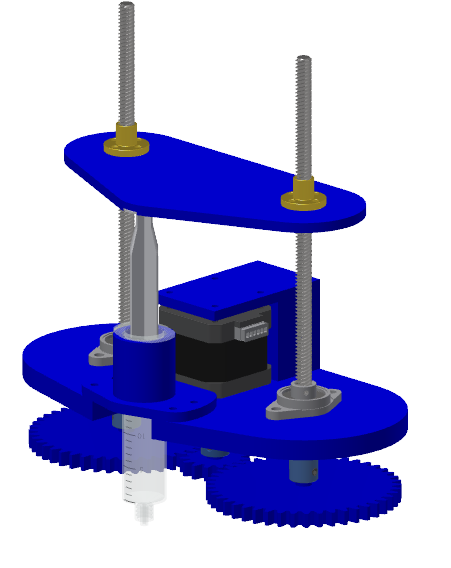
\includegraphics[scale=1]{figs/SyringeConcept1.png}
    \caption{Concept 1 Syringe-Based Extruder}
    \label{fig:extruderConcept1}
\end{figure}
\subsubsection*{Concept 2}
\begin{figure}[H]
    \centering
    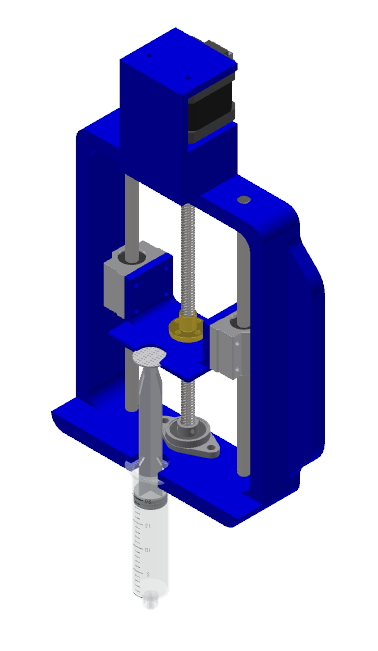
\includegraphics[scale=1]{figs/SyringeConcept2.png}
    \caption{Concept 2 Syringe-Based Extruder}
    \label{fig:extruderConcept2}
\end{figure}
\subsubsection*{Concept 3}
\begin{figure}[H]
    \centering
    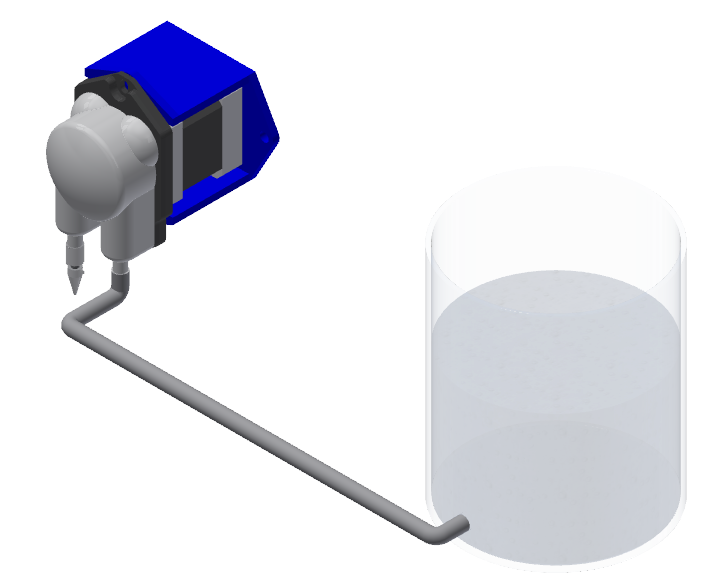
\includegraphics[scale=1]{figs/PumpConcept.png}
    \caption{Concept 3 Pump-Based Extruder}
    \label{fig:extruderConcept3}
\end{figure}
\subsection{Concept Evaluation and Selection}
\subsection{Final Design}


\section{Gantry Design}
\subsection{Concept Generation}
\subsubsection*{Concept 1}
\subsubsection*{Concept 2}
\subsection{Concept Evaluation and Selection}
\subsection{Final Design}


\section{Final Assembled Bioprinter}
\chapter{Embedded System Design}

\section{System Description}

\section{Hardware Design and Implementation}
\subsection{Hardware Block Diagram and Description of Interaction}
\subsection{Power Supply}
\subsection{Memory Storage and Programmer Circuit}
\subsection{Stepper Motor Setup}
\subsection{Load Cell Circuit}
\subsection{Thermocouple Circuit}
\subsection{FET Switching Circuit}

\section{Software Design and Implementation}

\section{Measurements and Results}



\chapter{Experimental Design}

\section{Materials and Methods}
\subsection{Materials}
The experimental setup requires the following equipment and materials:
\begin{itemize}
\item GelMA premix solution
\item Custom 3D printer with syringe-based extruder
\item Load cell
\item Computer
\item Measuring tape
\item Digital vernier caliper
\end{itemize}

The bioprinter is made up of an extruder, gantry, and curing system. A UV source is used to irradiate the GelMA prints to induce curing. The extruder uses a leadscrew to extrude the GelMA out of a syringe (onto a glass bed) that is wrapped in alumium foil (to prevent premature curing), and the force is measured using a load cell and sampled using an STM32 microcontroller. The extruder position is varied with a gantry that uses belts to adjust the extruder position along the horizontal plain and uses a lead screw to adjust the nozzle offset.

The bioprinter’s printing parameters are adjusted using a computer which behaves as an interface and the prints produced in each trial of the experiment are measured using a measuring tape and digital vernier caliper. This experimental setup is shown below in Figure~\ref{fig:experimentalSetup}:
 \begin{figure}[h]
    \centering
    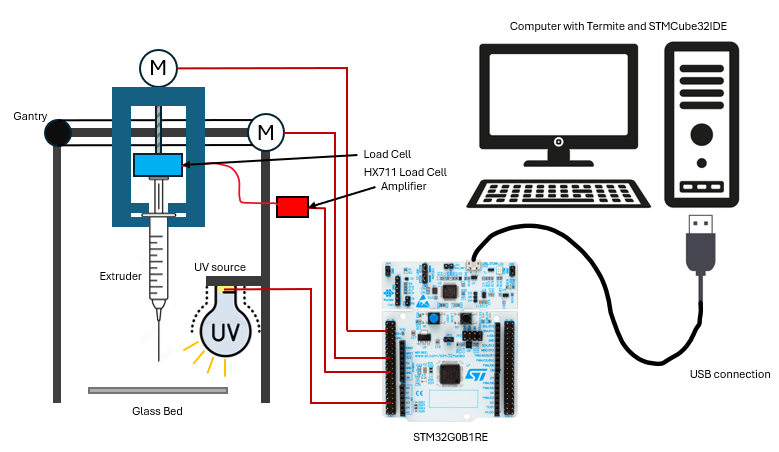
\includegraphics[scale=0.7]{figs/ExperimentalSetup.png}
    \caption{Experimental Setup (please change pic)}
    \label{fig:experimentalSetup}
\end{figure}

\subsection{Equipment Specifications}
The experimental equipment needs to allow a 10mm line of GelMA to be extruded onto a printing bed where the print line’s width and can be measured at points along the line without distorting the print line’s dimensions over the course of the measurement process as this would decrease the reliability of the measurements. The experiment also needs a way to configure the bioprinter’s parameters and receive real time printing feedback.


\subsubsection*{GelMA Specifications}

The Gelatin Methacrylate premix solution consists of GelMA and Irgacure 2959 (a photoinitiator that gives the solution its curing ability), which are dissolved in a solvent known as Phosphate Buffered Saline (PBS). The final composition is 10\% w/v GelMA with 0.1\% w/v Irgacure 2959 in PBS. The GelMA premix must be stored at 4\,\textdegree{}C, protected from UV light (to prevent premature curing) by wrapping its container in aluminium foil, and used to print within 2 weeks of preparation \citep{gelma_protocol}.

\subsubsection*{Bioprinter Specifications}

\begin{itemize}
    \item \textbf{Load cell} – A 50\,kg load cell is mounted to the extruder and is used with an HX711 load cell amplifier, which conditions the signal and sends it to the printer’s controller (STM32G0B1RE) via a digital output and clock terminal. The purpose of the load cell is to provide real-time measurement (through Termite) of the extrusion force to monitor for extrusion risks such as clogging, which is identified by irregularly high extrusion forces.
    
    \item \textbf{Extruder} – This consists of a syringe with a volume of 10\,ml and a nozzle diameter of 1\,mm. A leadscrew with a 2\,mm pitch is driven by a NEMA 17 stepper motor to extrude the GelMA out of the syringe.
    
    \item \textbf{Gantry} – The gantry is used to position the extruder in 3D space. Two NEMA 17 stepper motors drive belts that control the 2-axis motion in the horizontal plane. A leadscrew (also driven by a NEMA 17) with a 2\,mm pitch is used to control the extruder’s vertical position.
    
    \item \textbf{Bed} – The GelMA is printed on a 15\,mm $\times$ 15\,mm glass bed.
    
    \item \textbf{Curing system} – This comprises a UV LED that shines ultraviolet light with a wavelength of 365\,nm for 5 minutes after printing \cite{gelma_protocol}, ensuring the size and shape of the print remains stable and does not change during measurement.
\end{itemize}

\subsubsection*{Software}

\begin{itemize}
    \item \textbf{STM32CubeIDE} – The IDE is used to configure the printing parameters by adjusting the code that the STM32G0B1RE runs.

    \item \textbf{Termite} – The STM32G0B1RE sends real-time measurement data of the extruder position, bed temperature, and extrusion force via UART communication. This data is received and displayed by Termite through a USB cable. This is useful for real-time monitoring of each print and ensures smooth operation of the bioprinter.

    \item \textbf{MATLAB} – The data obtained from manually measuring the print width and height can be processed and plotted using MATLAB.
\end{itemize}


\subsection{Methods}
The variables identified in this experiment are shown below in Table~\ref{tab:variables}:
\begin{longtable}{|>{\raggedright\arraybackslash}p{4cm}|>{\raggedright\arraybackslash}p{10cm}|}
\caption{Experimental Variables} \label{tab:variables} \\
\hline
\textbf{Variable Type} & \textbf{Variables} \\
\hline
\endfirsthead

\hline
\textbf{Variable Type} & \textbf{Variables} \\
\hline
\endhead

Independent Variables & Extrusion rate, Printing speed, Nozzle height \\
Dependent Variables   & Extrusion force, Layer height, Layer width, Print quality \\
Controlled Variables  & GelMA concentration, Nozzle diameter \\
Extraneous Variables  & Ambient temperature, Vibrations \\
\hline
\end{longtable}


During the analysis of results, the mean layer height and width, as well as the standard deviation of the layer height and width (in mm) along each of the 10\,mm printed lines, are tabulated against the varied printing parameters: extrusion rate (mm/s), printing speed (mm/s), and nozzle height (mm). The two standard deviations serve as separate measures of print quality, where high deviations indicate lower print stability and quality.

The extrusion force from the load cell, measured via the COM port using MATLAB, is also plotted against time for each of the four different extrusion rates. The nozzle diameter affects both the speed and width of the extruded gel, influencing the resulting line width, height, and quality. These dependent variables are also affected by the rheological properties of the GelMA, which is why nozzle diameter and GelMA concentration are kept constant as controlled variables.

Ambient temperature and environmental vibrations, including those from the printer itself, can also influence outcomes. However, these are considered extraneous variables and are not within the scope of control in this experiment.

\subsubsection*{Experimental Setup Procedure}

Before the experiment can be conducted, the following setup procedure must be followed:

\begin{enumerate}
    \item Remove the GelMA premix from storage.
    \item Slowly load the GelMA premix solution into the syringe by fully submerging the syringe nozzle into the solution and pulling the plunger to minimize air bubbles in the loaded syringe. Air bubbles can compromise print quality by causing sudden breaks in the printed line.
    \item Allow the loaded syringe to sit for one hour to reach room temperature, reducing viscosity and aiding in air bubble removal. Then hold the syringe vertically with the nozzle facing upwards and flick the syringe to float any remaining bubbles to the top. Carefully push the plunger until hydrogel begins to extrude.
    \item Wrap the extruder in aluminium foil to prevent premature curing inside the syringe.
    \item Load the syringe into the bioprinter.
    \item Connect the printer to power.
    \item Use STM32CubeIDE and Termite to configure controller settings. Ensure the load cell reads zero and is scaled correctly using a known calibration weight.
    \item Connect the STM32G0B1RE to the computer via USB cable.
    \item Verify that both MATLAB and Termite are configured to read live data from the correct COM port.
\end{enumerate}

\subsubsection*{Test Procedure}

Once the setup is complete, the following test procedure is performed:

\begin{enumerate}
    \item Use STM32CubeIDE to vary the extrusion rate (mm/s), printing speed (mm/s), and nozzle offset (mm).
    \item Begin the extrusion process to deposit a 10\,mm long GelMA line onto the bed. Monitor the print using Termite.
    \item Use MATLAB to acquire and process the time-based extrusion force data for each extrusion rate.
    \item After printing, if no UV shielding is present, evacuate the room while the UV light cures the print for 5 minutes.
    \item Re-enter the room and measure the printed line’s width and height at 10 equidistant points (1\,mm apart) using a digital caliper.
    \item Record the mean and standard deviation of the 10 measurements for both width and height. These serve as metrics for print stability and quality.
    \item Repeat each test condition three times. Compute 95\% confidence intervals for each of the four measured variables (mean and standard deviation of width and height) to quantify measurement uncertainty and evaluate repeatability.
\end{enumerate}

A proposed test matrix is shown in Table~\ref{tab:testmatrix}, which outlines the combination of printing parameters for each trial in the experiment.

\begin{longtable}{ccc}
\caption{Proposed Test Matrix for Each Experiment} \label{tab:testmatrix} \\
\hline
\textbf{Test No.} & \textbf{Printing Speed (mm/s)} & \textbf{Extrusion Speed (mm/s)} \\
\hline
1  & 1 & 0.025 \\
2  & 1 & 0.050 \\
3  & 1 & 0.075 \\
4  & 1 & 0.100 \\
5  & 2 & 0.025 \\
6  & 2 & 0.050 \\
7  & 2 & 0.075 \\
8  & 2 & 0.100 \\
9  & 3 & 0.025 \\
10 & 3 & 0.050 \\
11 & 3 & 0.075 \\
12 & 3 & 0.100 \\
13 & 4 & 0.025 \\
14 & 4 & 0.050 \\
15 & 4 & 0.075 \\
16 & 4 & 0.100 \\
\hline
\end{longtable}
These tests are split up into two experiments, two compare the variation of nozzle offset. In experiment A, the nozzle offset is set to 2mm and in experiment B, it is set to 4mm.

\section{Discussion of Results and Conclusion}
Each test is iterated 3 times. This means that the 16 tests performed for each nozzle height (2 in total) will be iterated 3 times, yielding a total of 96 tests in total. The mean (across the 3 iterations) for the four measured variables per test will be calculated and tabulated in Table 3 below for each nozzle height.

{\small
\begin{longtable}{>{\raggedright\arraybackslash}p{1cm} 
                  >{\centering\arraybackslash}p{2cm} 
                  >{\centering\arraybackslash}p{2cm} 
                  >{\centering\arraybackslash}p{1.5cm} 
                  >{\centering\arraybackslash}p{1.5cm} 
                  >{\centering\arraybackslash}p{1.5cm}
                  >{\centering\arraybackslash}p{1.5cm}}
\caption{Results Table Template}  \label{tab:results} \\
\hline

\textbf{Test No.} & \textbf{Print Speed (mm/s)} & \textbf{Extrusion Speed (mm/s)} & \textbf{Mean Width (mm)} & \textbf{Mean Height (mm)} & \textbf{Std Dev Width (mm)} & \textbf{Std Dev Height (mm)} \\
\hline
\endhead
\hline
1  & 1 & 0.025 & -- & -- & -- & -- \\
2  & 1 & 0.050 & -- & -- & -- & -- \\
3  & 1 & 0.075 & -- & -- & -- & -- \\
4  & 1 & 0.100 & -- & -- & -- & -- \\
5  & 2 & 0.025 & -- & -- & -- & -- \\
6  & 2 & 0.050 & -- & -- & -- & -- \\
7  & 2 & 0.075 & -- & -- & -- & -- \\
8  & 2 & 0.100 & -- & -- & -- & -- \\
9  & 3 & 0.025 & -- & -- & -- & -- \\
10 & 3 & 0.050 & -- & -- & -- & -- \\
11 & 3 & 0.075 & -- & -- & -- & -- \\
12 & 3 & 0.100 & -- & -- & -- & -- \\
13 & 4 & 0.025 & -- & -- & -- & -- \\
14 & 4 & 0.050 & -- & -- & -- & -- \\
15 & 4 & 0.075 & -- & -- & -- & -- \\
16 & 4 & 0.100 & -- & -- & -- & -- \\
\hline
\end{longtable}
}


The tabulated data is used to determine the combination of print parameter for each printing speed that yields print lines with the best quality (lowest standard deviation of height and width). Confidence intervals for all 4 dependent variables, can be calculated from the three iterations.

These intervals will be tabulated in two more tables (identical to Table~\ref{tab:results}). They will be used to determine the uncertainty from random errors, which will be evaluated to determine the repeatable of the experiment.

After the uncertainty analysis, the extrusion force for each of the four extrusion rates can be plotted against time in seconds on a single plot using MATLAB. This may provide valuable information in characterising the rheological properties of the GelMA premix solution that can be used to determine new combinations of printing parameters for test matrices used in future versions of this experiment.

The successful completion of this experiment will produce a quantified relationship between print quality and the various printing parameters of the GelMA 3D bioprinter as well as provide information that will be useful for determining different print parameter ranges in future iterations of the experiment. The produced information will be used to produce more accurate and high-quality prints in the field of tissue engineering.
\chapter{Conclusions}


\appendix%------------------------------------------------------------
\chapter{Calculations}

\section{Syringe Calculations}

\textbf{Given:}
\begin{align*}
\text{Inner diameter of barrel (ID}_1\text{)} &= \SI{20}{\milli\meter} \\
\text{Length of barrel (L}_1\text{)} &= \SI{80}{\milli\meter} \\
\text{Inner diameter of nozzle (ID}_2\text{)} &= \SI{0.2}{\milli\meter} \\
\text{Length of nozzle (L}_2\text{)} &= \SI{20}{\milli\meter}
\end{align*}

\textbf{Cross-sectional areas:}
\begin{align*}
A_1 &= \pi \left(10 \times 10^{-3}\right)^2 \approx 314 \times 10^{-6} \, \si{\meter\squared} \\
A_2 &= \pi \left(0.1 \times 10^{-3}\right)^2 \approx 31.4 \times 10^{-9} \, \si{\meter\squared}
\end{align*}

\textbf{Max extrusion speed at nozzle:}
\[
v = \SI{5}{\milli\meter\per\second} = 5 \times 10^{-3} \, \si{\meter\per\second}
\]

\textbf{Volumetric flow rate:}
\[
Q = v \cdot A_2 = (5 \times 10^{-3}) \cdot (31.4 \times 10^{-9}) = 1.57 \times 10^{-10} \, \si{\meter\cubed\per\second}
\]

\textbf{Assumed viscosity:} 
\[
\mu = \SI{10}{\pascal\second}
\]

\textbf{Poiseuille's Law:}
\[
\Delta P = \frac{8 \mu L Q}{\pi r^4}
\]

\textbf{Total pressure required:}
\begin{align*}
P_B &= P_{\text{atm}} = \SI{101325}{\pascal} \\
P_A &= \frac{8 \cdot 10 \cdot 0.08 \cdot (1.57 \times 10^{-10})}{\pi (0.01)^4}
+ \frac{8 \cdot 10 \cdot 0.02 \cdot (1.57 \times 10^{-10})}{\pi (0.0001)^4}
+ 101325 \\
&= \SI{900919}{\pascal} = \SI{900.919}{\kilo\pascal}
\end{align*}

\textbf{Required force:}
\[
F = P \cdot A_1 = (900\,919) \cdot (314 \times 10^{-6}) = \SI{282.889}{\newton}
\]

\textbf{Design force (with safety margin):}
\[
F_{\text{design}} = \SI{300}{\newton}
\]

\chapter{Experimental results}


\backmatter%----------------------------------------------------------
\bibliography{bib/bib-sample}
 
\end{document}   

